\begin{figure}[ht]
  \centering
  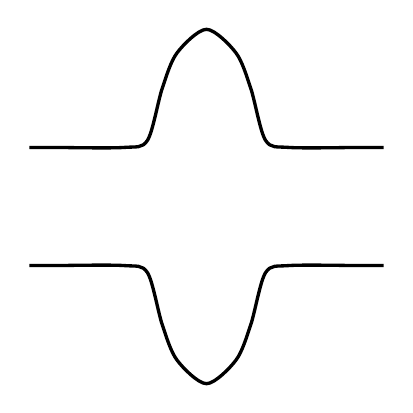
\begin{tikzpicture}[scale=1.5]
    \draw [very thick] plot [smooth] coordinates {(0,1) (0.2, 1) (0.8, 1) (1, 1.06)
      (1.125, 1.5) (1.25, 1.8) (1.5, 2) (1.75, 1.8) (1.875, 1.5) (2, 1.06) (2.2, 1)
      (2.8, 1) (3, 1)};

    \draw [very thick] plot [smooth] coordinates {(0,0) (0.2, 0) (0.8, 0) (1, -0.06)
      (1.125, -0.5) (1.25, -0.8) (1.5, -1) (1.75, -0.8) (1.875, -0.5) (2, -0.06) (2.2, 0)
      (2.8, 0) (3, 0)};
    
  \end{tikzpicture}
  \caption[A radio-frequency cavity.]{A representation of a radio-frequency
    cavity where the electric field lines are shown in black.}
  \label{fig:rf-cavity}
\end{figure}
